\documentclass[11pt]{article}

% Change "review" to "final" to generate the final (sometimes called camera-ready) version.
% Change to "preprint" to generate a non-anonymous version with page numbers.
\usepackage[final]{acl}
\usepackage{adjustbox}
\usepackage{multirow}
\definecolor{lightgray}{gray}{0.95}
\usepackage{booktabs}
\usepackage{colortbl}
\usepackage{xcolor}
\usepackage[ruled,vlined]{algorithm2e}
\usepackage{xspace}
\usepackage{amssymb}
\newcommand{\projectname}{\textsc{DocOCR-Eval}\xspace}
\newcommand{\yifan}[1]{\textcolor{red}{[Yifan: #1]}}
\newcommand{\yihao}[1]{\textcolor{red}{[Yihao: #1]}}
% Standard package includes
\usepackage{times}
\usepackage{latexsym}

% For proper rendering and hyphenation of words containing Latin characters (including in bib files)
\usepackage[T1]{fontenc}
% For Vietnamese characters
% \usepackage[T5]{fontenc}
% See https://www.latex-project.org/help/documentation/encguide.pdf for other character sets

% This assumes your files are encoded as UTF8
\usepackage[utf8]{inputenc}

% This is not strictly necessary, and may be commented out,
% but it will improve the layout of the manuscript,
% and will typically save some space.
\usepackage{microtype}

% This is also not strictly necessary, and may be commented out.
% However, it will improve the aesthetics of text in
% the typewriter font.
\usepackage{inconsolata}

%Including images in your LaTeX document requires adding
%additional package(s)
\usepackage{graphicx}

% If the title and author information does not fit in the area allocated, uncomment the following
%
%\setlength\titlebox{<dim>}
%
% and set <dim> to something 5cm or larger.

\title{\projectname: A Correction-Based Framework for OCR Tool Selection Without Ground Truth}

% Author information can be set in various styles:
% For several authors from the same institution:
% \author{Author 1 \and ... \and Author n \\
%         Address line \\ ... \\ Address line}
% if the names do not fit well on one line use
%         Author 1 \\ {\bf Author 2} \\ ... \\ {\bf Author n} \\
% For authors from different institutions:
% \author{Author 1 \\ Address line \\  ... \\ Address line
%         \And  ... \And
%         Author n \\ Address line \\ ... \\ Address line}
% To start a separate ``row'' of authors use \AND, as in
% \author{Author 1 \\ Address line \\  ... \\ Address line
%         \AND
%         Author 2 \\ Address line \\ ... \\ Address line \And
%         Author 3 \\ Address line \\ ... \\ Address line}

\author{
  \textbf{Zihan Xu\textsuperscript{1}},
  \textbf{Puzhen Wu\textsuperscript{2}},
  \textbf{Lawrence Chun Man Lau\textsuperscript{3}}, \\
  \textbf{Wei Liu\textsuperscript{4}}, 
  \textbf{Sirui Li\textsuperscript{5}},
  \textbf{Yifan Peng\textsuperscript{6}},
  \textbf{Yihao Ding\textsuperscript{4}}
\\
\\
  \textsuperscript{1}University of Melbourne,
  \textsuperscript{2}The University of Hong Kong, 
  \textsuperscript{3}The University of Hong Kong, \\
  \textsuperscript{4}University of Western Australia,
  \textsuperscript{5}Murdoch University,
  \textsuperscript{6}Weill Cornell Medicine
\\
  \small{
    \textbf{Correspondence:} \href{mailto:email@domain}{yihao.ding@uwa.edu.au}
  }
}

%\author{
%  \textbf{First Author\textsuperscript{1}},
%  \textbf{Second Author\textsuperscript{1,2}},
%  \textbf{Third T. Author\textsuperscript{1}},
%  \textbf{Fourth Author\textsuperscript{1}},
%\\
%  \textbf{Fifth Author\textsuperscript{1,2}},
%  \textbf{Sixth Author\textsuperscript{1}},
%  \textbf{Seventh Author\textsuperscript{1}},
%  \textbf{Eighth Author \textsuperscript{1,2,3,4}},
%\\
%  \textbf{Ninth Author\textsuperscript{1}},
%  \textbf{Tenth Author\textsuperscript{1}},
%  \textbf{Eleventh E. Author\textsuperscript{1,2,3,4,5}},
%  \textbf{Twelfth Author\textsuperscript{1}},
%\\
%  \textbf{Thirteenth Author\textsuperscript{3}},
%  \textbf{Fourteenth F. Author\textsuperscript{2,4}},
%  \textbf{Fifteenth Author\textsuperscript{1}},
%  \textbf{Sixteenth Author\textsuperscript{1}},
%\\
%  \textbf{Seventeenth S. Author\textsuperscript{4,5}},
%  \textbf{Eighteenth Author\textsuperscript{3,4}},
%  \textbf{Nineteenth N. Author\textsuperscript{2,5}},
%  \textbf{Twentieth Author\textsuperscript{1}}
%\\
%\\
%  \textsuperscript{1}Affiliation 1,
%  \textsuperscript{2}Affiliation 2,
%  \textsuperscript{3}Affiliation 3,
%  \textsuperscript{4}Affiliation 4,
%  \textsuperscript{5}Affiliation 5
%\\
%  \small{
%    \textbf{Correspondence:} \href{mailto:email@domain}{email@domain}
%  }
%}

\begin{document}
\maketitle
\begin{abstract}
Document parsing is a foundational step for document understanding tasks such as visual question answering and key information extraction, as it transforms unstructured scanned images into structured representations by extracting textual, visual, and layout information. While numerous Optical Character Recognition (OCR) engines and multimodal large language models (MLLMs) have been developed for this purpose, selecting an appropriate document parsing solution for a given document collection remains challenging, particularly in label-scarce settings. In this work, we conduct a systematic evaluation of text recognition performance across a diverse set of OCR engines and state-of-the-art MLLMs on multiple scanned document benchmarks spanning different domains and languages. Motivated by the limited contextual reasoning capabilities of many OCR engines and the high cost of manual annotations, we propose \textbf{\projectname}, an annotation-free evaluation framework for automatic OCR assessment and selection. \projectname employs a three-staged correction and ranking strategy to approximate annotation-based tool ordering without ground-truth labels. We show that aggregating across multiple MLLMs progressively improves alignment with annotation-based rankings. Extensive experiments further demonstrate that reliable OCR tool selection can be achieved in realistic, label-limited settings, providing practical guidance for deploying document parsing systems across diverse real-world document collections.
\end{abstract}

\section{Introduction}

The need to understand visually rich scanned documents has arisen in many domains, including finance \cite{formnlu}, education \cite{vies}, and healthcare \cite{rxpad}. These documents are typically distributed as scanned images with complex layouts that combine text, visual elements, and structural cues, and are often affected by scanning noise and distortion. To support downstream tasks such as visual question answering \cite{docvqa,mmvqa} and key information extraction (KIE) \cite{sroie,ding2025synjac}, document parsing is required to convert unstructured images into structured representations by extracting textual, visual, and layout information.

%
%Numerous OCR engines \cite{cui2025paddleocr30technicalreport,easyocr_2023} and vision-language models \cite{chatgpt,gemini1.5} have been developed for parsing scanned documents, achieving strong performance across diverse benchmarks. However, selecting an appropriate tool for a target document collection is typically done empirically or relies on additional human annotations for evaluation. An automatic and cost-efficient approach to domain-specific tool selection is therefore crucial for downstream document understanding, particularly in agentic application settings.

\begin{table*}[ht]
\centering
\caption{Comparison of OCR engines, document parsing APIs, and vision-language models for document understanding.}
\footnotesize
% \scriptsize
%\setlength{\tabcolsep}{3pt}
%\begin{adjustbox}{max width=\textwidth}
\resizebox{\textwidth}{!}{%
\begin{tabular}{l l l l l l l l l}
\toprule
\textbf{Tool Name} & \textbf{Provider} & \textbf{Deployment} & \textbf{Pricing} & \textbf{Input Formats} & \textbf{Languages} & \textbf{Openness} & \textbf{GPU} & \textbf{Doc Parsing} \\
\midrule
\rowcolor{gray!20}\multicolumn{9}{l}{OCR Engine}\\
SuryaOCR~\cite{paruchuri2025surya} & Datalab & Local & Free & Image, PDF, Word, PPT & 90+ & Open & Optional & No \\
Kraken~\cite{kraken_ocr_2025} & Inria et al. & Local & Free & Image, PDF & Multi & Open & Optional & No \\
olmOCR~\cite{olmocrbench} & AI2 & Hybrid & Free & Image, PDF & Multi & Open & Required & Yes \\
AttentionOCR~\cite{Zhang2019-attention} & Guo \& Deng & Local & Free & Image & Multi & Open & Optional & No \\
Calamari~\cite{wick_calamari_2020} & Univ. Würzburg & Local & Free & Image & Multi & Open & Optional & No \\
EasyOCR~\cite{easyocr_2023} & JaidedAI & Local & Free & Image & 80+ & Open & Optional & No \\
Tesseract~\cite{tesseract_ocr_5} & S. Weil & Local & Free & Image & 100+ & Open & Not Required & No \\

PaddleOCR~\cite{cui2025paddleocr30technicalreport} & PaddlePaddle & Cloud & Free & Image, PDF & 80 & Open & Optional & Yes \\
docTR~\cite{doctr2021} & Mindee & Local & Free & Image, PDF & Multi & Open & Optional & No \\
Ocular~\cite{ocular_ocr} & Berkeley NLP & Local & Free & Image, PDF & Multi & Open & Optional & No \\
Google Cloud Vision~\cite{google_cloud_vision_ocr} & Google & Cloud & Paid & Image, PDF & 220+ & Closed & Not Required & Yes \\
%  & 
 \midrule

\rowcolor{gray!20}\multicolumn{9}{l}{MLLM} \\
LightOnOCR~\cite{lightonocr2025}& LightOnAI & Cloud & Paid & Image, PDF & 2 & Closed & Required & No \\
Qwen3-VL~\cite{Qwen3-VL} & Aliyun & Hybrid & Free & Image, PDF & 32 & Closed & Required & No \\
OpenAI Vision~\cite{openai_vision_api} & OpenAI & Cloud & Paid & Image, PDF & Multi & Closed & Not Required & Yes \\
DeepSeek-OCR~\cite{wei2025deepseek} & DeepSeek AI & Hybrid & Paid & Image, PDF & Multi & Open-source & Supported & No \\
HunyuanOCR~\cite{hunyuanvisionteam2025hunyuanocrtechnicalreport} & Tencent & Local & Free & Image, PDF & 100+ & Open-source & Supported & No \\
Seed-VL~\cite{seed2025seed1_5vl} & ByteDance Seed & Cloud & Paid & Image, PDF & Multi & Open-source & Supported & Yes \\
\bottomrule
\end{tabular}
%\end{adjustbox}
}
\label{tab:ocr_llm_comparison}
\end{table*}
% Document parsing tool summary
OCR engines primarily focus on detecting and recognizing text from document images. They are typically open-sourced and freely available, but require non-image formats (e.g., PDF, Word, PowerPoint) to be converted into images prior to processing (Table~\ref{tab:ocr_llm_comparison}). While Optical Character Recognition (OCR) systems can extract text along with bounding boxes, often at the text-line level, they rely mostly on vision-based backbones trained in an object detection style. As a result, they are prone to missing text, spelling mistakes, and syntactic errors, which can propagate through OCR-dependent document understanding frameworks \cite{luo2024layoutllm, ding2025survey}. 

Recent multimodal large language models (MLLMs) offer an alternative by leveraging contextual reasoning for more robust text extraction, but they typically incur higher computational costs and rely on cloud-based deployment. Moreover, many MLLM-based methods generate plain-text outputs without explicit spatial boundaries, limiting their capability for layout-aware downstream systems and increasing the risk of hallucinations. 

Existing document understanding frameworks often rely on fixed or ad-hoc choices of parsing tools, overlooking the rapid evolution of both OCR engines and MLLM-based approaches. Moreover, evaluating text recognition performance typically requires costly manual annotations, which limit scalable and adaptive tool selection in real-world deployments. In practice, tool selection must balance recognition accuracy with resource constraints, such as annotation effort, computational overhead, and deployment cost.

To address this challenge, we propose an automated and cost-efficient framework for selecting the most suitable document-parsing tool for a given scanned document collection. The main contributions of this work are summarized as follows: 
%
\textbf{First}, we systematically evaluate conventional OCR engines and state-of-the-art MLLMs on representative scanned document benchmarks, providing a thorough cross-model and cross-domain comparison on text recognition.
%
\textbf{Second}, we propose \projectname, an annotation-free evaluation workflow that enables reliable cross-domain tool selection without requiring ground-truth labels.
%
\textbf{Finally}, we validate the effectiveness and robustness of \projectname across diverse document domains and languages, demonstrating its practical applicability in real-world settings.


\section{\textsc{DocOCR-Eval} Pipeline}
\subsection{Problem Definition} 
Given a document collection $\mathbb{D} = \{D_i\}_{i=1}^N$ from a specific domain and a set of $K$ candidate OCR engines $\mathcal{P} = \{p_j\}_{j=1}^K$, our goal is to automatically identify the engine $p \in P$ that yields the best overall performance on $\mathbb{D}$ without relying on human-annotated ground truth (GT). The selected OCR engine is then used to support downstream document parsing tasks, either by providing textual input to OCR-dependent frameworks or by serving as supervision for training OCR-free document understanding models.
\subsection{\projectname}
\begin{figure*}[t]
    \centering
    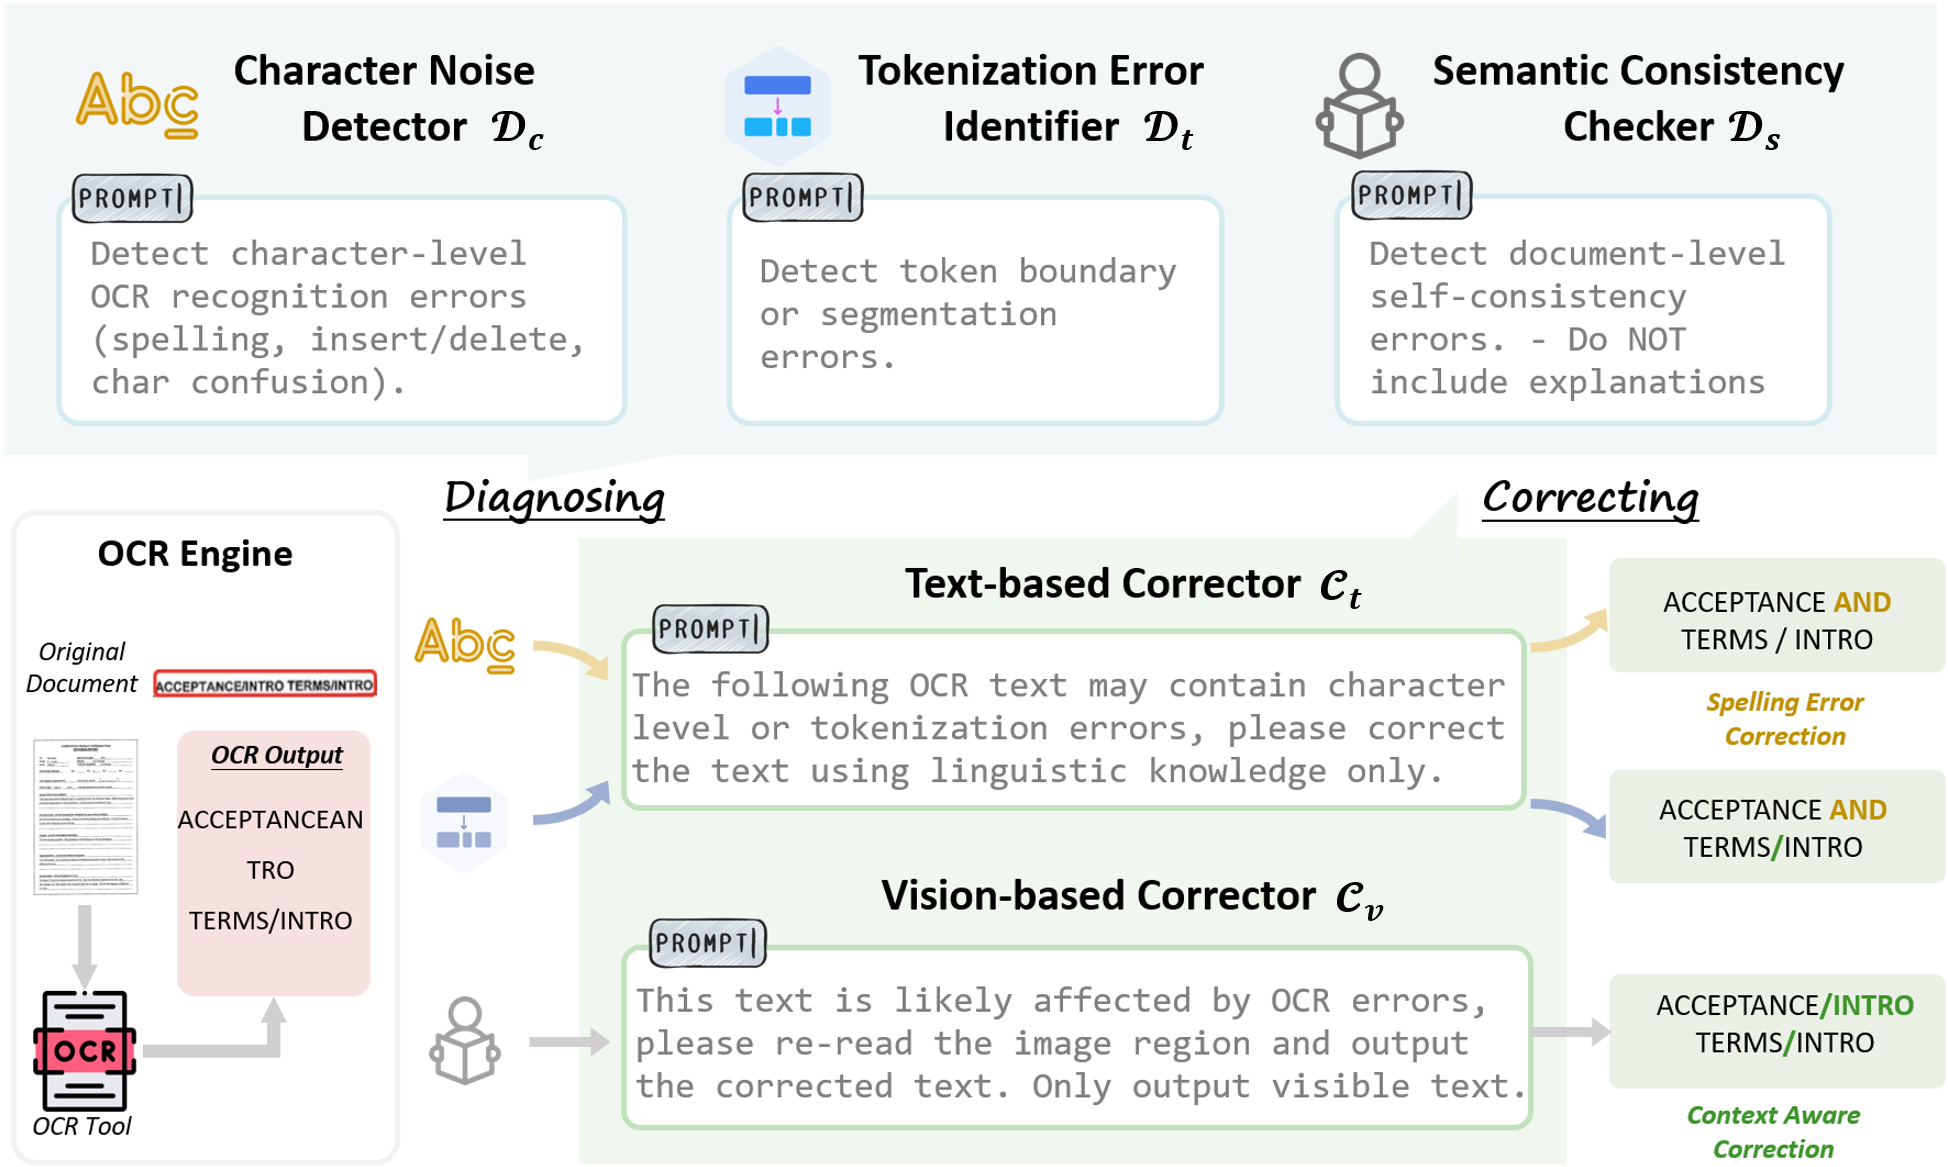
\includegraphics[width=0.8\linewidth]{figure/method_sigir_ocr.png}
    \caption{Workflow of the \projectname with a case study.}
    \label{fig:workflow}
\end{figure*}
We propose an annotation-free OCR engine selection pipeline that evaluates OCR quality by measuring the discrepancy between original OCR outputs and their corresponding corrections generated by an MLLM. 

For each document, the OCR output is processed through two stages: \emph{Error Diagnosing} and \emph{Error Correcting}.
By aggregating discrepancy scores over the entire document collection, we rank candidate OCR engines and select the one with the minimal overall discrepancy as the most suitable for deployment.

\subsubsection{Error Diagnosing Modules} 

These modules aim to diagnose various error types in the original OCR outputs (Figure~\ref{fig:workflow}). Given a document $D$, an OCR engine first extracts text and generates an output $T$. Each OCR output block $t \in T$ is then processed by three diagnosing modules. The Character Noise Detector ($\mathcal{D}_c$) detects character-level errors, including substitutions, insertions, deletions, and visually confusable glyphs. The Tokenization Error Identifier ($\mathcal{D}_t$) detects segmentation errors, such as incorrect word boundaries, whitespace errors, and line-break artifacts. The Semantic Consistency Checker ($\mathcal{D}_s$) assesses whether a text block is semantically inconsistent with the target document $D$. Each module outputs a binary decision, yielding a structured vector that enables fine-grained control over subsequent correction actions
$\mathbf{d}_k = [\mathcal{D}_c(t_k), \mathcal{D}_t(t_k), \mathcal{D}_s(t_k,D)]$.

\subsubsection{Error Correcting Modules}
We introduce two MLLM-based correction modules that leverage MLLM's rich commonsense knowledge and strong contextual reasoning.
The Text-based Corrector ($\mathcal{C}_t$) revises OCR outputs using linguistic and contextual cues alone, without introducing content beyond the recognized text. 
The Vision-based Corrector ($\mathcal{C}_v$) additionally incorporates the OCR bounding box cropped from the source image and instructs the MLLM to re-recognize only the visible text within that region.


\subsubsection{Error Diagnosis, Correction, and Ranking}

Based on the diagnostic signals from the error diagnosing modules ${\mathcal{D}_c,\mathcal{D}_t,\mathcal{D}_s}$, each OCR output block $t$ is conditionally corrected using the corresponding error correcting modules ${\mathcal{C}_t,\mathcal{C}_v}$.
Specifically, the Text-based Corrector $\mathcal{C}_t$ is applied when character-level or tokenization errors are detected, i.e., when $\mathcal{D}_c(t)=1$ or $\mathcal{D}_t(t)=1$. In contrast, the vision-based re-OCR corrector $\mathcal{C}_v$ is triggered for blocks exhibiting document-level semantic inconsistencies, indicated by $\mathcal{D}_s(t)=1$.

The staged correction yields post-correction outputs $\hat{T}_{D_i}^{(p_j)}$ for each OCR engine $p_j$ and document $D_i$. For single-MLLM correction, we compute Average Normalized Levenshtein Similarity (ANLS) scores $s_{j}$ for each engine and rank engines in descending order. To quantify the alignment between this correction-based ranking and the ground-truth ranking, we compute the Normalized Discounted Cumulative Gain (NDCG)~\cite{Wang2013-kb}, which assigns higher importance to top-ranked positions and progressively discounts lower-ranked items. Moreover, to mitigate potential bias from a single MLLM, we aggregate predictions from $k$ models by averaging their scores, $\bar{s}_{j}=\frac{1}{K}\sum_{k=1}^{K} s_{j}^{(k)}.$
\subsection{Experimental Setup}
\begin{table}[t]
\centering
\small
\setlength{\tabcolsep}{3pt}
\caption{Summary of adopted datasets. H: Handwritten. LA: Layout Analysis}
\label{tab:datasets_info}
\resizebox{\columnwidth}{!}{%
\begin{tabular}{l l l l r l}
\toprule
\textbf{Dataset} & \textbf{Language} & \textbf{Domain} & \textbf{H} & \textbf{Size} & \textbf{Proposed Tasks} \\
\midrule
FUNSD  & English   & Multiple              & Yes & 199  & OCR, LA, KIE \\
SROIE  & English   & Receipt               & No  & 1000 & OCR,  KIE \\
EPHOIE & Chinese   & Exam Paper & Yes & 1494 & OCR, KIE \\
RXPAD  & French    & Clinical Notes         & Yes & 200  & OCR, KIE \\
XFUND  & Multiple  & Multiple               & Yes & 1393 & OCR, LA, KIE \\
\bottomrule
\end{tabular}
}
\end{table}


\subsubsection{Dataset}
We evaluate OCR engines, MLLMs, and our OCR correction framework on five publicly available datasets covering diverse languages and domains: FUNSD~\cite{funsd} (general form understanding in English), SROIE~\cite{sroie}, EPHOIE~\cite{ephoie} (educational documents in Chinese), RXPAD~\cite{rxpad} (medical prescription documents in French), and XFUND~\cite{xu2022xfund} (Table~\ref{tab:datasets_info}). XFUND supports seven languages, each with 50 test images. To ensure fair and consistent evaluation across datasets of different sizes, we randomly sample 50 test images from each test split for all experiments. 
 


\subsubsection{Implementation Details}

Table~\ref{tab:ocr_llm_comparison} summarizes the key attributes of each tool. Using annotated datasets, we directly compare the predictions of PaddleOCR~\cite{cui2025paddleocr30technicalreport}, EasyOCR~\cite{easyocr_2023}, Tesseract~\cite{tesseract_ocr_5}, Google Cloud Vision~\cite{google_cloud_vision_ocr}, Qwen3-VL-Instruct-4B~\cite{Qwen3-VL}, and GPT-4.1-mini~\cite{gpt4o} against ground truth across multiple datasets. These tools represent diverse OCR paradigms, including open-source rule-based engines (Tesseract), deep-learning OCR engines (PaddleOCR, EasyOCR), widely deployed commercial cloud services (Google Cloud Vision), and recent MLLMs with unified visual-text reasoning (Qwen3-VL-Instruct-4B and GPT-4.1-mini). 

For annotation-free evaluation, we evaluate PaddleOCR, EasyOCR, Tesseract, and Google Cloud Vision using MLLM-driven correction. For each OCR block, we apply a three-stage error diagnosis with Qwen3-VL-4B-Instruct, Qwen3-VL-8B-Instruct, GPT-4.1-mini, and Gemini-2.5-flash-lite, which triggers text- or vision-based re-OCR when needed. All experiments were conducted on NVIDIA A100 GPUs with deterministic inference by setting the temperature to 0.0 and disabling sampling.


\subsubsection{Evaluation Metrics}
For text recognition Performance, we report ROUGE-L to measure consistency between predicted and reference text, Character Error Rate (CER) to quantify character-level recognition errors, and ANLS as a length-normalised similarity measure. We also report word-level F1 to assess token-level coverage and the practical usability of extracted text. 

For tool selection performance, we assess ranking consistency using NDCG ($d$) under stepwise correction with each individual corrector ($\mathcal{D}_c$, $\mathcal{D}_t$, $\mathcal{D}_s$), as well as their cascaded combinations ($\mathcal{D}_c+\mathcal{D}_t$ and $\mathcal{D}_c+\mathcal{D}_t+\mathcal{D}_s$). Finally, an average NDCG score ($Avg.d$) is presented for each dataset. Performance is further evaluated quantitatively using ANLS for both single-MLLM and multi-MLLM post-correction settings. 
 
\section{Results and Discussion}
%In this section, we report the text recognition results of representative OCR engines and MLLMs against ground-truth annotations, and evaluate the effectiveness of \textsc{DocOCR-Eval} in automatically selecting the most suitable tool for domain-specific documents.


\subsection{OCR Tool Performance}
\begin{table}[t]
\centering
\caption{ANLS of text recognition with ground-truth.}
\label{tab:ocr_comparison}

%\renewcommand{\arraystretch}{1.15}

\begin{adjustbox}{max width=\linewidth}
\begin{tabular}{lccccccccc}
\toprule
 & EPHOIE & FUNSD & SROIE & RXPAD & XF-ja & XF-es & XF-it & XF-de & XF-pt \\
\midrule
\rowcolor{gray!20}\multicolumn{10}{l}{OCR-engine-based}\\
PaddleOCR      & 0.20 & \textbf{0.42} & 0.51 & \textbf{0.66} & 0.46 & 0.83 & 0.34 & 0.88 & 0.88 \\
EasyOCR        & 0.09 & 0.29 & 0.35 & 0.61 & 0.53 & \textbf{0.87} & 0.74 & \textbf{0.90} & \textbf{0.90} \\
Tesseract      & 0.02 & 0.23 & 0.38 & 0.52 & 0.45 & 0.79 & 0.69 & 0.84 & 0.84 \\
Cloud Vision   & \textbf{0.44} & 0.29 & \textbf{0.56} & 0.29 & \textbf{0.62} & 0.73 & \textbf{0.75} & 0.74 & 0.74 \\
\midrule
\rowcolor{gray!20}\multicolumn{10}{l}{MLLM-based}\\
Qwen3-VL       & 0.46 & 0.29 & 0.53 & 0.28 & 0.48 & 0.59 & 0.46 & 0.70 & 0.70 \\
OpenAI         & 0.34 & 0.25 & 0.37 & 0.28 & 0.54 & 0.65 & 0.67 & 0.71 & 0.71 \\

\bottomrule
\end{tabular}
\end{adjustbox}
\vspace{-1em}
\end{table}

%\subsection{OCR Tool Performance with Ground-Truth Annotations}

We first present text recognition results of representative OCR engines and MLLMs compared against ground-truth annotations. Table~\ref{tab:ocr_comparison} shows that no single OCR engine consistently outperforms the others, indicating that performance is highly dataset-dependent and motivating the need for automatic OCR tool selection. For instance, PaddleOCR performs strongly on FUNSD and RXPAD, while EasyOCR is competitive on several XFUND language subsets. By contrast, Cloud Vision and Qwen3-VL generally perform better on multilingual or visually complex datasets, such as EPHOIE and XFUND-it.

%\subsubsection{Performance Across Multiple Metrics} 

%To comprehensively evaluate text recognition performance,
We then evaluate OCR results against ground truth across multiple metrics on EPHOIE, FUNSD, and RXPAD. Figure~\ref{fig:panel} shows that Cloud Vision API and OpenAI achieve higher ANLS and word-level F1, indicating stronger character- and word-level matching for non-English documents. In contrast, PaddleOCR often achieves lower CER and higher ROUGE, suggesting better lexical overlap and sequence-level fidelity.
\begin{figure}[t]
  \centering
  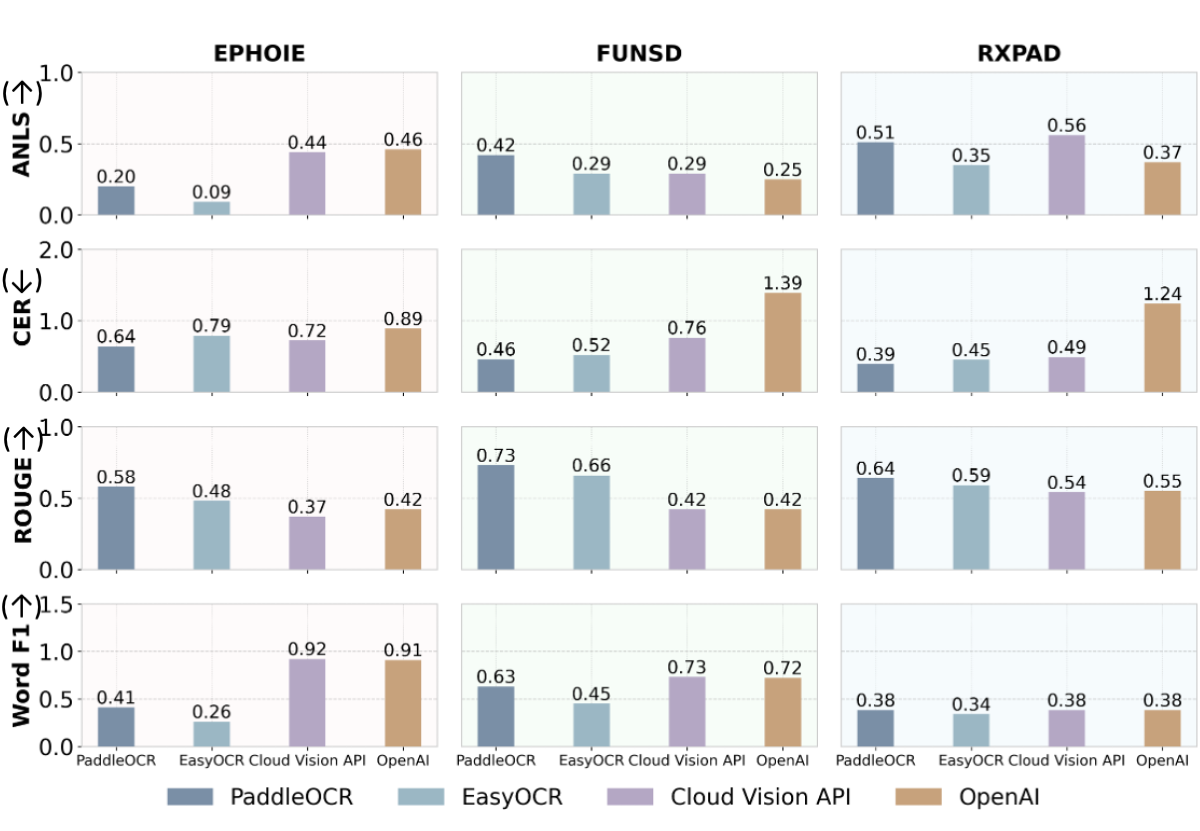
\includegraphics[width=1.0\linewidth,clip,trim=0 4em 0 0]{figure/metrics_panel.png}
  \caption{Metrics among diverse datasets by Qwen3-VL, $\uparrow$ higher is better; $\downarrow$ lower is better.}
  \label{fig:panel}
  \vspace{-1em}
\end{figure}

\subsection{Performance of Automatic Selection}
\subsubsection{Best-Performing Tool Identification} 

Next, we evaluate the effectiveness of \projectname in automatically selecting the most suitable tool for domain-specific document collections. Table~\ref{tab:average_mllm} shows the average scores from four MLLMs. Compared with the single-MLLM correction (upper table), averaging ANLS across multiple MLLMs improves top-1 selection accuracy and narrows the performance gap between the annotation-based top-selected tool (highlighted in green) and competing alternatives. In the table, green cells denote the ground-truth best tool, bold values indicate the tool selected by correction, and red cells mark disagreements with the ground truth. Although the corrected rankings do not perfectly match the annotation-based rankings, the score differences consistently decrease as more models are aggregated. This trend indicates that averaging mitigates individual model bias and variance and produces rankings that increasingly approximate the ground-truth annotation-based order.
%
\begin{table}[t]
\centering
%\small
\caption{Text recognition results after correction. Green cells: the annotation-based top-1 tool. Bold: the tool selected for correction. Red cells: disagreements with GT.}
\label{tab:average_mllm}
% ---------- Top table ----------
%\renewcommand{\arraystretch}{1.15}
\begin{adjustbox}{max width=\linewidth}
\begin{tabular}{lccccccccc}
\toprule
 & EPHOIE & FUNSD & SROIE & RXPAD & XF-ja & XF-es & XF-it & XF-de & XF-pt \\
 \midrule
\rowcolor{gray!20}\multicolumn{10}{l}{\textbf{Qwen3-VL post-correction ANLS}} \\
%\midrule
PaddleOCR      & 0.95 & \cellcolor{green!15}{\textbf{0.94}} & \cellcolor{red!15}{\textbf{0.95}} & \cellcolor{green!15}{\textbf{0.96}} & 0.92 & 0.97 & \cellcolor{red!15}{\textbf{0.98}} & \cellcolor{red!15}{\textbf{0.99}} & 0.95 \\
EasyOCR        & 0.47 & 0.82 & 0.90 & 0.92 & 0.87 & \cellcolor{green!15}{\textbf{0.98}} & 0.97 & \cellcolor{green!15}{0.97} & \cellcolor{green!15}{\textbf{0.96}} \\
Tesseract      & 0.56 & 0.64 & 0.93 & 0.88 & 0.58 & 0.92 & 0.93 & 0.96 & 0.91 \\
Cloud Vision   & \cellcolor{green!15}{\textbf{0.97}} & 0.88 & \cellcolor{green!15}{0.90} & 0.93 & \cellcolor{green!15}{\textbf{0.97}} & 0.95 & \cellcolor{green!15}{0.95} & 0.95 & 0.94 \\

% \end{tabular}
% \end{adjustbox}
% % ---------- Bottom table ----------
% \renewcommand{\arraystretch}{1.15}
% \begin{adjustbox}{max width=\linewidth}
% \begin{tabular}{lccccccccc}
\midrule
\rowcolor{gray!20}\multicolumn{10}{l}{\textbf{Average ANLS post-correction from multiple MLLMs}} \\
%\midrule
 % & EPHOIE & FUNSD & SROIE & RXPAD & XF-ja & XF-es & XF-it & XF-de & XF-pt \\
% \midrule
PaddleOCR  & 0.927 & \cellcolor{green!15}{\textbf{0.933}} & \cellcolor{red!15}{\textbf{0.945}} & \cellcolor{green!15}{\textbf{0.949}} & 0.767 & 0.941 & 0.946 & 0.949 & 0.910 \\
EasyOCR  & 0.467 & 0.805 & 0.890 & 0.888 & 0.747 & \cellcolor{green!15}{\textbf{0.953}} & 0.927 & \cellcolor{green!15}{\textbf{0.956}} & \cellcolor{green!15}{\textbf{0.939}} \\
Tesseract & 0.571 & 0.522 & 0.818 & 0.646 & 0.498 & 0.824 & 0.804 & 0.816 & 0.759 \\
Cloud Vision API & \cellcolor{green!15}{\textbf{0.949}} & 0.908 & \cellcolor{green!15}{0.912} & 0.928 & \cellcolor{green!15}{\textbf{0.940}} & 0.951 & \cellcolor{green!15}{\textbf{0.948}} & 0.951 & 0.935 \\
\bottomrule
\end{tabular}
\end{adjustbox}

\end{table}
\subsubsection{Ranking Consistency with ground truth} 

Table~\ref{tab:ranking_all_datasets} summarizes OCR engine rankings under annotation-based evaluation and our proposed stepwise correction framework, along with their rank alignment across datasets. Green cells indicate rankings consistent with the ground-truth order, while red cells denote discrepancies.
%
Overall, we observe moderate agreement between the two regimes under NDCG evaluation. On FUNSD ($Avg.d=0.9752$), correction-based rankings perfectly match annotation-based rankings, indicating that our framework can reliably recover relative performance without ground-truth labels. On more challenging datasets, alignment remains high but slightly reduced. EPHOIE achieves average NDCG values to 0.9679, while RXPAD reaches 0.9699, suggesting although exact rank matching may vary, the framework consistently preserves the most important top-ranked positions. 
%Across datasets, Cloud Vision exhibits the highest rank volatility, whereas PaddleOCR remains comparatively stable.


\begin{table}[t]
\centering
%\small
\caption{OCR engine rankings under stepwise correction across datasets by Qwen3-VL. Green cells: rankings consistent
with the ground-truth order. Red cells: discrepancies in rankings with the ground-truth order.}
\footnotesize
\setlength{\tabcolsep}{3pt}
\label{tab:ranking_all_datasets}
%\renewcommand{\arraystretch}{1.15}
\begin{adjustbox}{max width=\linewidth}
\begin{tabular}{
p{1.69cm}
>{\centering\arraybackslash}p{1cm}
>{\centering\arraybackslash}p{.95cm}
>{\centering\arraybackslash}p{.95cm}
>{\centering\arraybackslash}p{.95cm}
>{\centering\arraybackslash}p{.95cm}
>{\centering\arraybackslash}p{.95cm}
>{\centering\arraybackslash}p{.8cm}
}
\toprule
OCR Engine 
& GT Rank 
& $\mathcal{D}_c$
& $\mathcal{D}_t$
& $\mathcal{D}_s$
& $\mathcal{D}_c+\mathcal{D}_t$
& All 
& $Avg.d$ \\
\midrule

\rowcolor{gray!20}\multicolumn{8}{l}{EPHOIE}\\
PaddleOCR        & 2 & \cellcolor{red!15}{1} & \cellcolor{red!15}{1} & \cellcolor{green!15}{2} & \cellcolor{red!15}{1} & \cellcolor{green!15}{2} & \multirow{5}{*}{0.9679} \\
EasyOCR          & 3 & \cellcolor{green!15}{3} & \cellcolor{green!15}{3} & \cellcolor{green!15}{3} & \cellcolor{green!15}{3} & \cellcolor{red!15}{4} &  \\
Tesseract        & 4 & \cellcolor{green!15}{4} & \cellcolor{green!15}{4} & \cellcolor{green!15}{4} & \cellcolor{green!15}{4} & \cellcolor{red!15}{3} &  \\
Cloud Vision API & 1 & \cellcolor{red!15}{2} & \cellcolor{red!15}{2} & \cellcolor{green!15}{1} & \cellcolor{red!15}{2} & \cellcolor{green!15}{1} &  \\
$d$ & - & 0.9496 & 0.9496 & 1.0000 & 0.9496 & 0.9905 & \\
\midrule

\rowcolor{gray!20}\multicolumn{8}{l}{FUNSD}\\
PaddleOCR        & 1 & \cellcolor{green!15}{1} & \cellcolor{green!15}{1} & \cellcolor{red!15}{2} & \cellcolor{green!15}{1} & \cellcolor{green!15}{1} & \multirow{5}{*}{0.9752} \\
EasyOCR          & 3 & \cellcolor{red!15}{4} & \cellcolor{red!15}{4} & \cellcolor{green!15}{3} & \cellcolor{green!15}{3} & \cellcolor{green!15}{3} &  \\
Tesseract        & 4 & \cellcolor{red!15}{3} & \cellcolor{red!15}{3} & \cellcolor{green!15}{4} & \cellcolor{red!15}{2} & \cellcolor{green!15}{4} &  \\
Cloud Vision API & 2 & \cellcolor{green!15}{2} & \cellcolor{green!15}{2} & \cellcolor{red!15}{1} & \cellcolor{red!15}{4} & \cellcolor{green!15}{2} &  \\
$d$ & - & 0.9905 & 0.9905 & 0.9496 & 0.9543 & 1.0000 & \\
\midrule

\rowcolor{gray!20}\multicolumn{8}{l}{RXPAD}\\
PaddleOCR        & 1 & \cellcolor{red!15}{2} & \cellcolor{green!15}{1} & \cellcolor{green!15}{1} & \cellcolor{green!15}{1} & \cellcolor{green!15}{1} & \multirow{5}{*}{0.9699} \\
EasyOCR          & 2 & \cellcolor{red!15}{1} & \cellcolor{green!15}{2} & \cellcolor{red!15}{4} & \cellcolor{green!15}{2} & \cellcolor{red!15}{3} &  \\
Tesseract        & 3 & \cellcolor{green!15}{3} & \cellcolor{green!15}{3} & \cellcolor{green!15}{3} & \cellcolor{green!15}{3} & \cellcolor{red!15}{4} &  \\
Cloud Vision API & 4 & \cellcolor{green!15}{4} & \cellcolor{green!15}{4} & \cellcolor{red!15}{2} & \cellcolor{green!15}{4} & \cellcolor{red!15}{2} &  \\
$d$ & - & 0.9496 & 1.00 & 0.9543 & 1.00 & 0.9548 & \\
\bottomrule
\end{tabular}
\end{adjustbox}
\vspace{-2em}
\end{table}
We then examine the effect of each corrector. Table~\ref{tab:ranking_all_datasets} shows that optimal correction strategies vary across datasets. 
EPHOIE primarily benefits from context-aware re-reading (semantic correction $\mathcal{D}_s$), likely due to irregular layouts and semantic inconsistencies. 
FUNSD requires the full cascade, indicating heterogeneous error sources. 
In contrast, RXPAD favors text-only normalization ($\mathcal{D}_c + \mathcal{D}_t$), as domain-specific abbreviations make vision-based re-OCR prone to additional noise. 
These findings suggest that correction strategies should be dataset-adaptive rather than universally applied. %To obtain a more robust and generalizable estimate of correction performance, we therefore additionally report results averaged by multiple MLLMs.





%\subsubsection{Rank Alignment between Full-corrected and Annotation-based Rank} Table~\ref{tab:ranking_all_datasets} visualizes the rank differences between the two evaluation regimes, where positive values indicate an improvement in rank after correction and negative values indicate a decline. Overall, we observe substantial but imperfect rank alignment between annotation-based and correction-based rankings. For several datasets, such as FUNSD, rankings remain stable across all engines, suggesting that correction-based evaluation can reliably recover the same relative ordering of OCR systems as annotation-based evaluation, even in the absence of annotations. However, some datasets exhibit rank shifts. For example, SORIE and XFUND-it show larger deviations, indicating that post-correction disproportionately benefits or penalizes certain OCR systems depending on document characteristics and language. Across datasets, Cloud Vision API exhibits the largest rank volatility, whereas PaddleOCR shows comparatively stable rankings. Consistent with the observed rank stability across multiple datasets, correction-based ranking correctly identifies the top-one performing OCR engine in 66.7\% of cases when compared against annotation-based ranking.
%\begin{figure}[htbp]
%  \centering
%  \includegraphics[width=1.0\linewidth]{samples/figures/rank_heatmap.png}
%  \caption{Rank Alignment Between Anntation-based ranking and Correction-based ranking by ANLS}
%  \label{fig:heatmap}
%\end{figure}

%\subsubsection{Rank Alignment between Stepwise and Annotation-based Rank} After applying the proposed staged correction pipeline, we observe consistent and substantial improvements across all datasets and OCR engines (Table~\ref{tab:ocr_comparison}). Correction alters the relative ranking of OCR engines. For example, on EPHOIE and XFUND-ja, Cloud Vision achieves the highest post-correction scores, whereas PaddleOCR dominates on FUNSD and RXPAD after correction. This ranking shift demonstrates that correction effectiveness is not merely a function of the original OCR accuracy, but also of how amenable each engine’s errors are to structured diagnosis and targeted correction.


\subsection{Case Study}

To illustrate how the proposed staged correction framework operates in practice, we present a representative case study drawn from the FUNSD dataset. Figure~\ref{fig:workflow} shows an OCR output produced by PaddleOCR and the subsequent correction process guided by our staged diagnostic pipeline using Qwen3-VL-Instruct-4B.

The original OCR output contains the phrase ``ACCEPTANCE-ANTRO TERMS/INTRO'', where the intended text is ``ACCEPTANCE /INTRO TERMS/INTRO''. Although the overall semantic structure is preserved, the text exhibits multiple subtle OCR errors.
In Step 1, the model identifies character-level errors such as missing accents and visually confusable characters (e.g., ``ACCEPRANCE-ANTRO'' vs. ``ACCEPTANCE''). 
In Step 2, it detects tokenization and segmentation errors, such as incorrect word boundaries and malformed token sequences (e.g., ``TERMS/INTRO'' instead of ``TERMS / INTRO''). These two steps operate independently and produce structured binary signals indicating whether each error type is present.
In Step 3, the model evaluates the OCR block against its surrounding page context. In this example, the phrase is semantically inconsistent with the surrounding text. As a result, vision-based re-OCR is triggered. Qwen3-VL correctly finds ``ACCEPTANCE/INTRO'', not ``ACCEPTANCE AND '', and returns the final corrected texts.

\subsection{Latency, Cost and Performance Trade Off}
%While the proposed correction-based evaluation pipeline demonstrates strong potential for annotation-free OCR tool selection, several practical considerations should be acknowledged when deploying such a pipeline in real-world settings. First, inference time remains a critical factor. Although staged correction enables fine-grained diagnosis and targeted re-OCR, it introduces additional computational overhead compared to directly using raw OCR outputs. MLLMs incur substantially higher latency than traditional OCR engines. For large-scale document collections or time-sensitive applications, the trade-off between improved recognition quality and increased processing time must be carefully balanced. Second, user requirements and downstream task sensitivity play an important role in determining whether correction is warranted. In applications such as document retrieval or coarse-grained indexing, minor recognition errors may have a limited impact, and lightweight OCR solutions may suffice. Finally, cost tolerance and resource constraints influence the feasibility of correction-based tool selection. Commercial OCR APIs and large vision–language models typically involve usage-based pricing or significant hardware requirements. Users and organizations must therefore consider whether the performance gains achieved through correction justify the additional financial and computational costs. In this sense, correction should be viewed not as a universal replacement for OCR evaluation, but as a configurable component that can be selectively applied based on budget, scale, and accuracy requirements.
While the proposed correction-based pipeline shows potential for annotation-free OCR tool selection, it introduces additional latency, because MLLMs are substantially slower than traditional OCR engines. Its usefulness therefore depends on downstream task requirements. For retrieval or coarse-grained indexing, lightweight OCR may suffice, whereas correction is better suited to high-accuracy settings. Moreover, commercial APIs and large vision–language models incur monetary or hardware costs, so users must balance performance gains against resource constraints. Accordingly, correction should be treated as a configurable option rather than a default solution.
\section{Conclusion}

This paper presents an annotation-free framework for OCR tool selection through a staged error detection and correction using MLLMs. By systematically comparing traditional OCR engines and MLLMs across multiple datasets, we demonstrate that correction-based evaluation can recover reliable tool rankings and identify top-performing systems without ground-truth annotations.


% Bibliography entries for the entire Anthology, followed by custom entries
%\bibliography{anthology,custom}
% Custom bibliography entries only
\bibliography{sigir2026}

%\appendix

%\section{Example Appendix}
%\label{sec:appendix}

%This is an appendix.

\end{document}
